
\section{CAP y PACELC en RabbitMQ}

\begin{frame}{CAP: Consistencia, Disponibilidad, Particiones}
  \small
  \begin{itemize}
    \item \textbf{Consistencia (C):} las lecturas que se realizan deben reflejar el estado más reciente de los datos.
    \item \textbf{Disponibilidad (A):} el sistema responde a cada solicitud con una respuesta válida.
    \item \textbf{Tolerancia a particiones (P):} el sistema debe afrontar interrupciones de comunicación entre sus nodos.
  \end{itemize}

  \begin{block}{¿Dónde está el problema?}
    Si los nodos dejan de comunicarse, el sistema puede tener que limitar algunas operaciones para mantener la consistencia, o seguir respondiendo con menos garantías.
  \end{block}

 \begin{block}{Ejemplo: quorum queue de RabbitMQ}
    Una cola replicada en tres miembros necesita
    una mayoría de dos para operar.

    Si uno queda aislado, la mayoría puede
    continuar; la minoría no puede confirmar
    publicaciones de forma independiente.
  \end{block}

  {\tiny Fundamento CAP: \cite{ahmed2023,myrhorodskyi2025}.
  Comportamiento de RabbitMQ: \cite{rabbitmq2026quorum}.}
\end{frame}

\begin{frame}{PACELC: consistencia frente a latencia}
  \small
  \begin{itemize}
    \item \textbf{Si hay una partición (P):} se presenta el compromiso entre la disponibilidad y la consistencia.
    \item \textbf{Si no hay una partición (E):} mantener las réplicas coordinadas solo para mantener la consistencia puede hacer que aumente la latencia.
  \end{itemize}

  \begin{block}{Aplicación a RabbitMQ}
    Las quorum queues utilizan consenso entre
    sus miembros, la necesidad de alcanzar
    una mayoría limita las operaciones cuando
    se pierde el quórum.
  \end{block}

  {\tiny Fundamento PACELC: \cite{ahmed2023,myrhorodskyi2025}.
  Caso RabbitMQ: \cite{rabbitmq2026quorum}.}
\end{frame}

\begin{frame}{Dos formas de procesar un pedido}
  \centering

  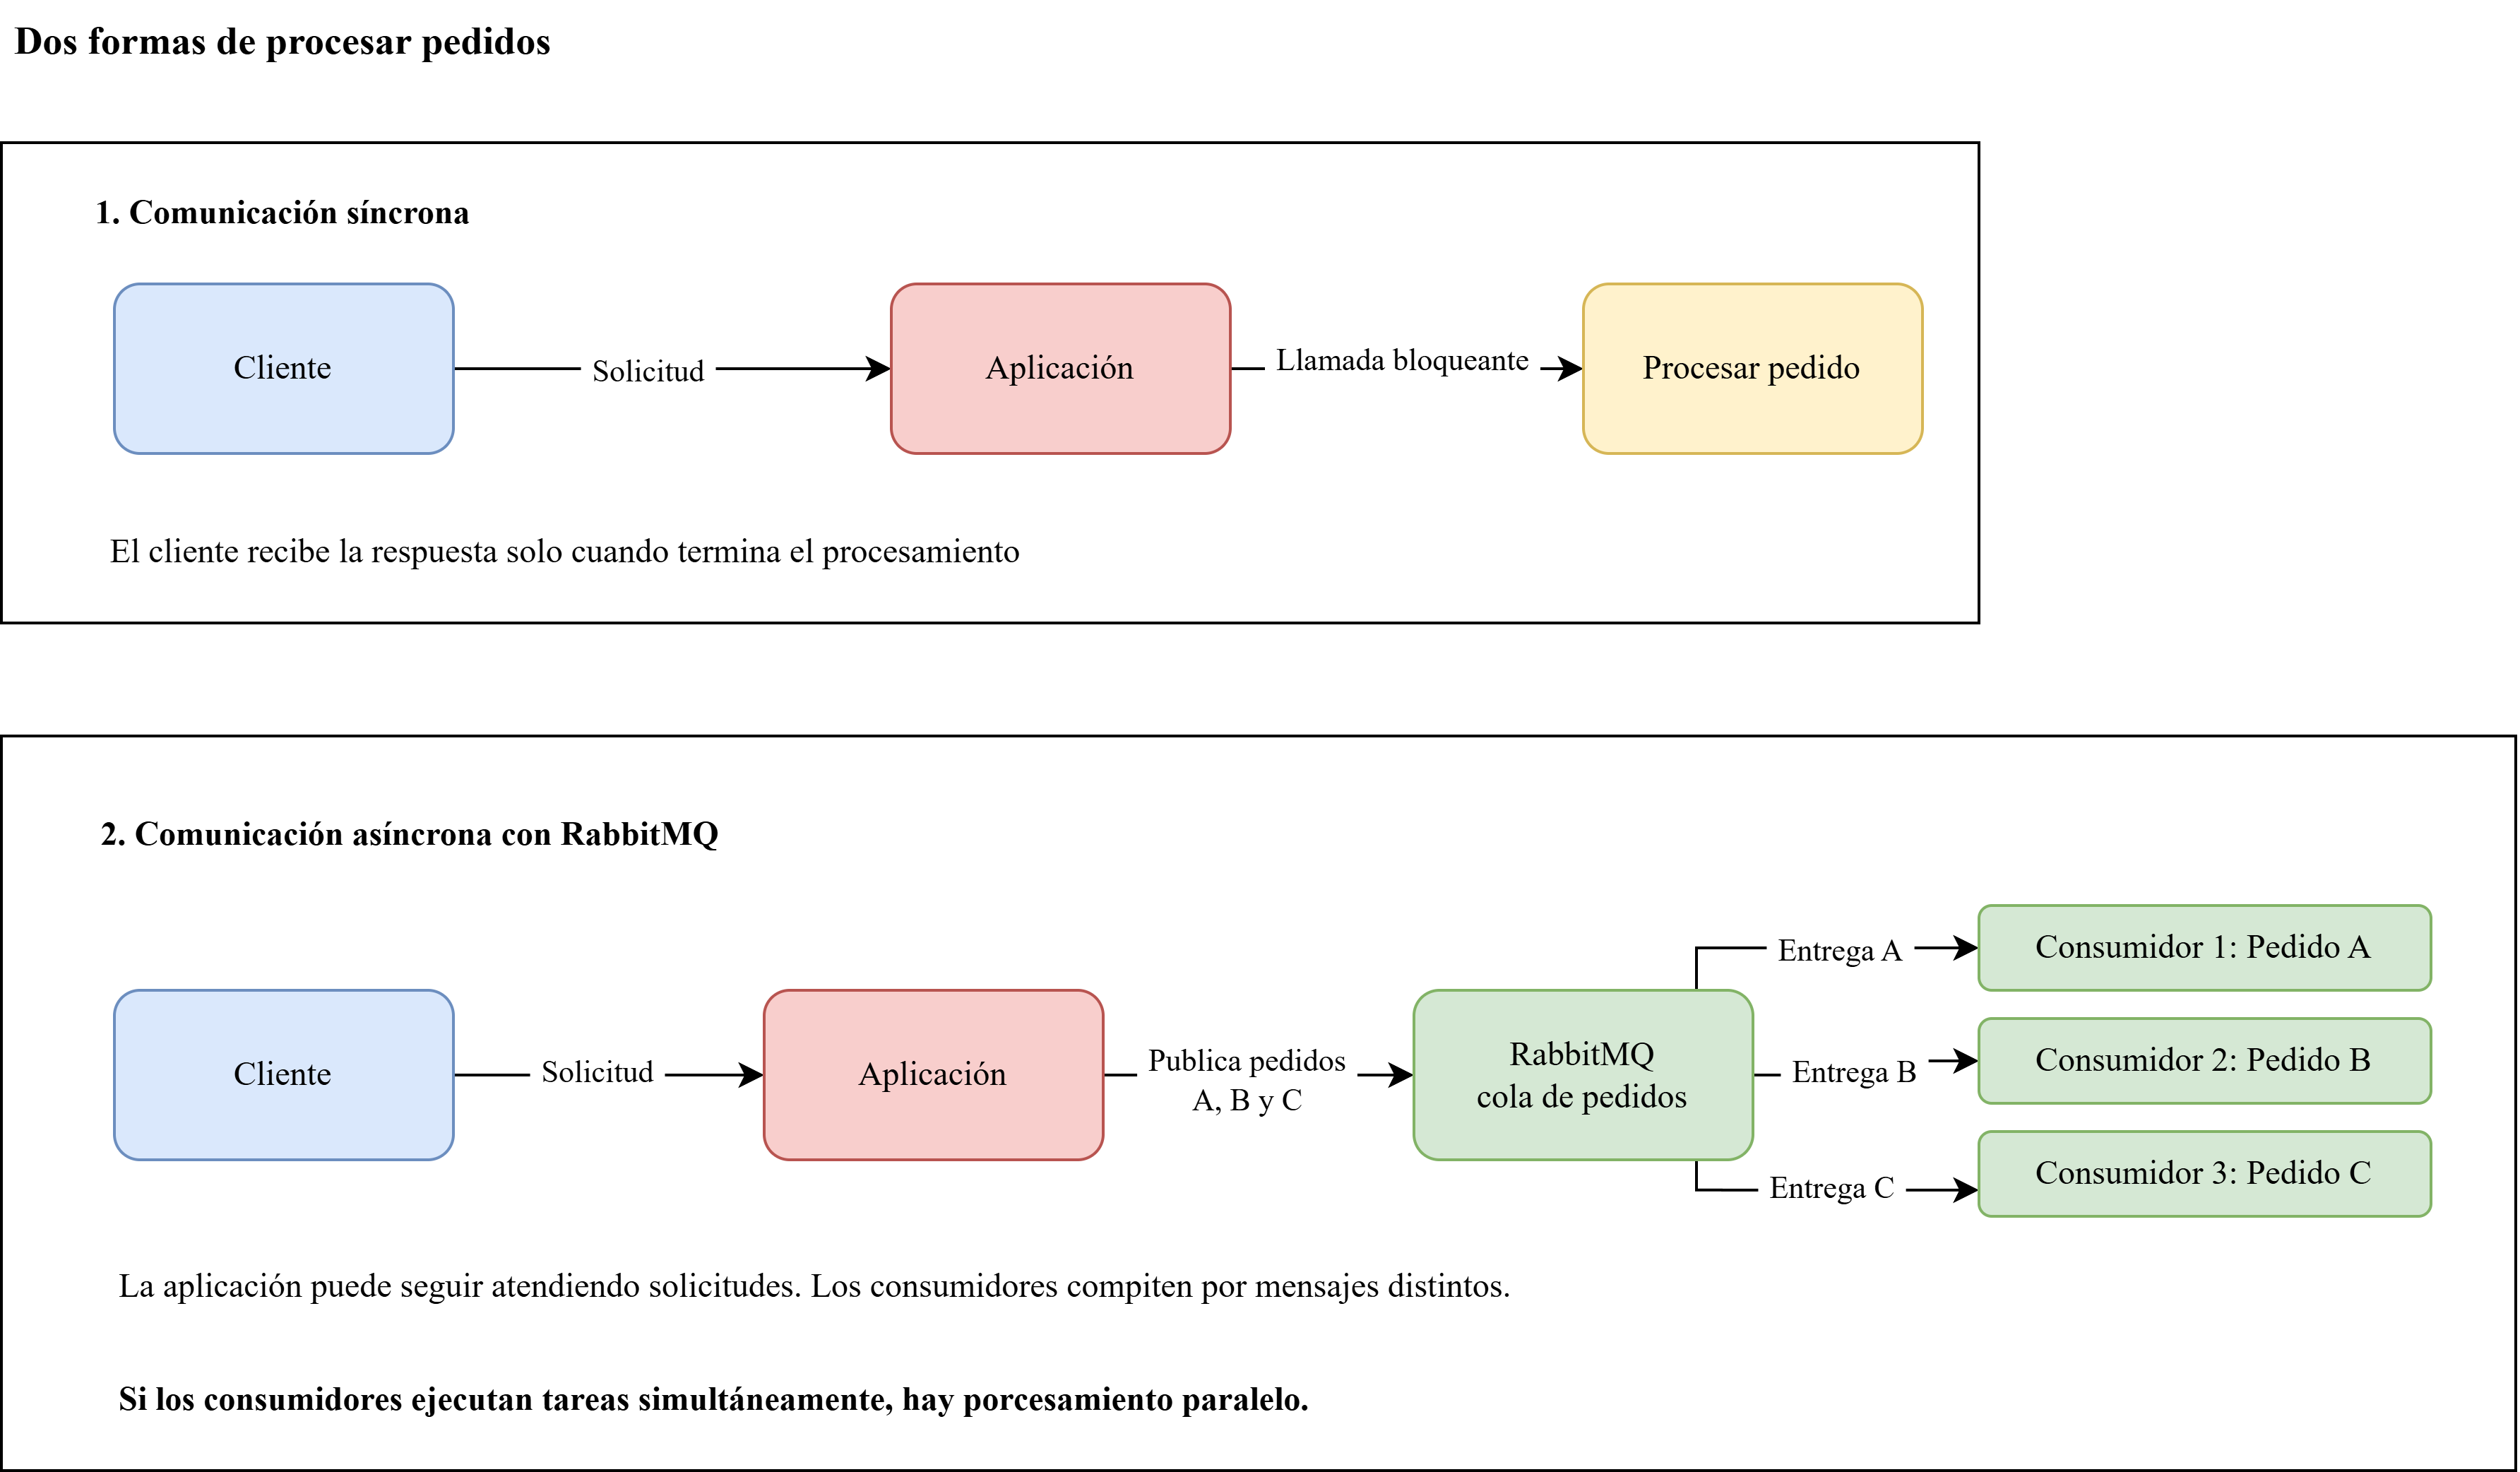
\includegraphics[
    width=0.96\textwidth,
    height=0.76\textheight,
    keepaspectratio
  ]{diagramas/procesamiento.png}

  \vspace{0.1cm}
  {\tiny Elaboración propia. Ejemplo de comunicación síncrona y asíncrona. A partir de \cite{maharjan2023,derlatka2023}. Nota: Los consumidores comparten la cola y
  procesan pedidos diferentes.}
  \end{frame}